% =============================================================================
% capitulos/cap2_hardware.tex
%   Cap. 2 -- Requisitos e arquitetura para a aquisição de imagens em campo
%   Versão consolidada (4 seções + introdução de capítulo)
% =============================================================================
\chapter{Requisitos e arquitetura para a aquisição de imagens em campo}
\label{cap:hardware}


Este capítulo define o subsistema de aquisição de imagens que precede o \textit{pipeline} de visão computacional. A discussão é organizada em quatro etapas: caracterização operacional dos pontos de alimentação do Campus 2 (Seção~\ref{sec:cap2-pontos}); requisitos mínimos e desejáveis do módulo de captura (Seção~\ref{sec:cap2-requisitos}); comparação entre as tipologias de câmera hoje disponíveis (Seção~\ref{sec:cap2-tipologias}); e a arquitetura recomendada para o Campus 2, com a respectiva justificativa e consequências para o \textit{pipeline} do Capítulo~\ref{cap:pipeline} (Seção~\ref{sec:cap2-arquitetura}). O detalhamento de \textit{datasheets}, dimensionamento e alternativas exploradas em pilotos paralelos é remetido ao Apêndice~\ref{ap:hardware}.


\section{Pontos no Campus 2}
\label{sec:cap2-pontos}


A discussão parte dos dez pontos de alimentação operados no Campus 2 da USP São Carlos, não de um cenário idealizado. O levantamento foi conduzido em campo por inspeções cooperativas junto aos voluntários da AEX Gatos do C2, combinando ficha técnica, registro fotográfico georreferenciado e observação direta da rotina de alimentação, procedimento alinhado às práticas de \textit{camera trapping} cooperativo, em que o conhecimento operacional dos cuidadores é informação primária \cite{velez2022choosing,cordier2022africa}. A matriz consolidada P01--P10 (Apêndice~\ref{ap:matriz-pontos}) reúne os atributos de campo; aqui sintetizam-se apenas os que condicionam o problema de software.


\begin{figure}[!htb]
  \centering
  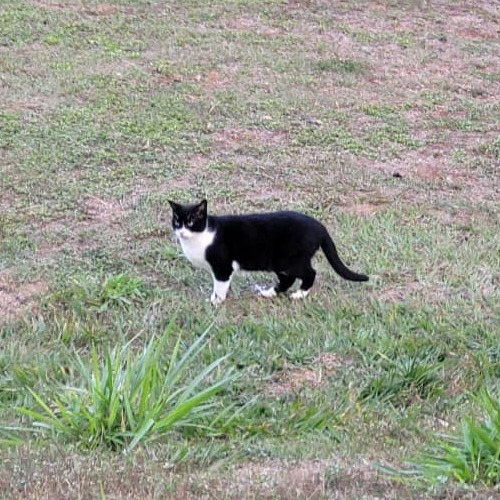
\includegraphics[width=0.24\linewidth]{elementos/figuras/cap2-gato1.jpeg}\hfill
  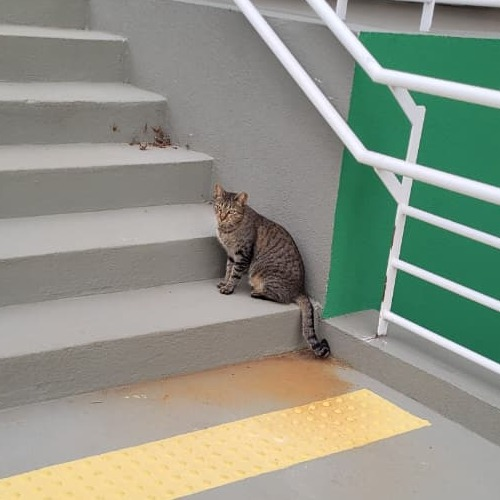
\includegraphics[width=0.24\linewidth]{elementos/figuras/cap2-gato2.jpeg}\hfill
  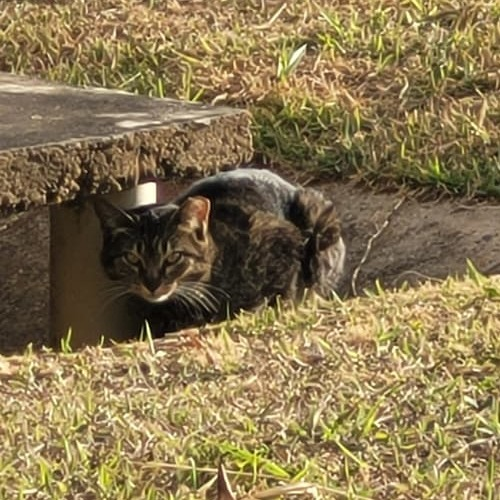
\includegraphics[width=0.24\linewidth]{elementos/figuras/cap2-gato3.jpeg}\hfill
  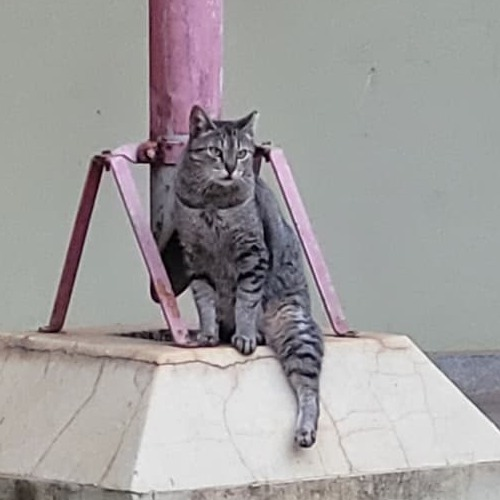
\includegraphics[width=0.24\linewidth]{elementos/figuras/cap2-gato4.jpeg}
  \caption[Diversidade fenotípica e de contexto ambiental na colônia do Campus 2.]
  {Indivíduos da colônia do Campus 2, ilustrando os desafios práticos para a identificação. As capturas evidenciam não apenas a diversidade de padrões de pelagem (sólido preto, \textit{tabby} cinza, bicolor branco e padrão mesclado), mas também variações nas poses dos animais, diferentes condições de iluminação associadas aos períodos do dia e a multiplicidade de ambientes encontrados pelo campus. Essa heterogeneidade visual reforça a necessidade e o papel da reidentificação automática descrita no Capítulo~\ref{cap:pipeline}.}
  \label{fig:diversidade-gatos}
  \fonte{Acervo do autor, \the\year.}
\end{figure}


Três eixos delimitam o problema de aquisição. O primeiro é \emph{físico}: os abrigos reciclados são estruturas adaptadas pelos voluntários, com caixas plásticas, telhas de fibrocimento, madeira recuperada e potes domésticos, dispostas no solo com geometria, altura e orientação variáveis. A infraestrutura é não padronizada; o módulo de captura precisa ser retrofitável a essas estruturas, sem obra civil e com baixo impacto visual. O segundo é \emph{energético e comunicacional}: sete dos dez pontos não dispõem de tomada de corrente alternada em raio operacionalmente útil (cerca de 20\,m), o que inviabiliza alimentação por rede elétrica como solução abrangente; em contrapartida, nove pontos recebem mais de quatro horas de incidência solar direta por dia (exceção do P05, em corredor coberto). A rede Wi-Fi institucional e a 4G alcançam nominalmente todos os pontos, mas a literatura adverte que disponibilidade nominal não equivale a estabilidade sustentada em ambiente externo arborizado \cite{bruce2025largescale,velez2022choosing}, ressalva que motiva a opção por arquitetura \textit{offline-first}.


O terceiro eixo é \emph{ecológico} e tem consequência algorítmica direta. Por estarem dispostos no solo, os potes atraem fauna não-alvo recorrente: gambás (\textit{Didelphis albiventris}), quatis (\textit{Nasua nasua}), lagartos teiú, pombos, aves nativas e felinos silvestres como o gato-mourisco (\textit{Herpailurus yagouaroundi}), cuja presença em fragmentos urbanos da região central do estado de São Paulo é documentada em revisões recentes de fauna sinantrópica \cite{goncalves2025wildcat,cove2022capital}. Essa biodiversidade altera o problema de software: não basta detectar presença diante do pote, é preciso discriminar a espécie antes de submeter o quadro às etapas seguintes. O emprego de modelos generalistas como o SpeciesNet \cite{google_speciesnet_blog} e a pilha MegaDetector com PyTorch-Wildlife \cite{hernandez2024pytorchwildlife,microsoft_cameratraps_repo} responde a essa observação.


\section{Requisitos do subsistema de aquisição}
\label{sec:cap2-requisitos}


Os requisitos do módulo de captura são separados em mínimos, sem os quais o \textit{pipeline} é inviável, e desejáveis, que diferenciam uma solução adequada à escala e à rotina da AEX Gatos do C2.


Os requisitos mínimos são cinco. O primeiro é o acionamento autônomo por movimento, por sensor infravermelho passivo (PIR) em \textit{hardware} ou por detecção de variação de pixels em \textit{software}. A gravação contínua é inviável em escala plurianual, pois \textit{ghost frames} acionados por vento, sombra ou variação térmica espúria respondem por metade ou mais do volume bruto capturado \cite{bruce2025largescale,velez2022choosing,swanson2015snapshot}. O segundo é a vedação ambiental classe IP66 ou superior, dada a exposição a chuva, orvalho, poeira e variação térmica diária acima de 15\,$^\circ$C. O terceiro é a autonomia energética compatível com pontos sem corrente alternada. O quarto é o armazenamento local suficiente para o regime \textit{offline-first} entre ciclos de coleta. O quinto é a captura noturna por infravermelho próximo (NIR), pois parte da atividade da colônia é crepuscular e noturna.


Aos mínimos somam-se dois requisitos desejáveis. O primeiro é a capacidade de processamento na borda (\textit{Edge AI}), com inferências leves que descartam quadros sem animal, filtram vegetação em movimento e rejeitam fauna não-alvo antes da transmissão, conforme implantações recentes \cite{velasco2024smartcameratraps,pishdast2025smartcameratraps,mulero2025addressing}. O segundo é a conectividade nativa para sincronização opcionalmente intermitente, que dispensa coleta manual sistemática de cartões e habilita a validação humana no laço. Esses dois requisitos determinam o quanto do \textit{pipeline} pode ser deslocado para a borda em vez de operar inteiramente em servidor.


A geometria com que a câmera observa o ponto precede qualquer escolha de modelo, pois determina o que é possível extrair do quadro. Dois conjuntos de \textit{features} precisam ser preservados em fração significativa dos quadros: a face do animal, relevante para abordagens face a face habilitadas pelo \textit{dataset} PetFace, e o flanco, incluindo padrão de pelagem, contorno corporal e marcação de orelha (\textit{ear-tipping}), conforme o método de reidentificação (re-ID) por partes do corpo de \citeonline{akbar2025bodypart}. A literatura aponta que alturas baixas, próximas ao nível dos ombros do animal, maximizam taxa de detecção e qualidade da identificação individual, ao passo que posicionamentos elevados, adotados como medida antifurto, reduzem tanto a probabilidade de disparo quanto a utilidade dos quadros \cite{seidlitz2020height,beukes2025refining,meek2016higher}. Ângulos levemente picados, com linha de visada apontada para o entorno imediato dos potes, oferecem o melhor compromisso entre cobertura do cone útil, captura simultânea de face e flanco e minimização de obstrução por vegetação rasteira \cite{beukes2025refining,moll2020viewshed}. A Figura~\ref{fig:posicionamento-camera} resume esse arranjo.


\begin{figure}[!htb]
  \centering
  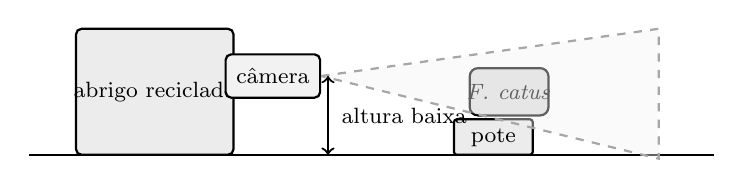
\begin{tikzpicture}[
      x=1cm, y=1cm,
      every node/.style={font=\footnotesize},
      box/.style={draw, thick, rounded corners=2pt, fill=gray!10,
                  minimum width=1.8cm, minimum height=0.8cm, align=center},
      cone/.style={draw=gray!70, thick, dashed, fill=gray!10, fill opacity=0.4},
      ground/.style={draw, thick}
    ]
    % Linha do solo
    \draw[ground] (-0.2,0) -- (8.5,0);

    % Abrigo (à esquerda)
    \draw[thick, fill=gray!15, rounded corners=2pt] (0.4,0) rectangle (2.4,1.6);
    \node at (1.4,0.8) {abrigo reciclado};

    % Câmera embutida no abrigo
    \node[box, minimum width=1.2cm, minimum height=0.55cm] (cam) at (2.9,1.0) {câmera};

    % Pote
    \draw[thick, fill=gray!15, rounded corners=1pt] (5.2,0) rectangle (6.2,0.45);
    \node at (5.7,0.22) {pote};

    % Animal-alvo (silhueta simples)
    \draw[thick, fill=gray!25, rounded corners=3pt]
      (5.4,0.5) rectangle (6.4,1.1);
    \node at (5.9,0.8) {\textit{F. catus}};

    % Cone de visão
    \draw[cone] (cam.east) -- (7.8,1.6) -- (7.8,-0.05) -- cycle;

    % Anotação de altura
    \draw[<->, thick] (3.6,0) -- (3.6,1.0);
    \node[right] at (3.65,0.5) {altura baixa};
  \end{tikzpicture}
  \caption[Esquema do posicionamento da câmera junto ao abrigo reciclado.]
  {Posicionamento de referência da câmera junto ao abrigo reciclado: altura baixa, próxima ao nível dos ombros do animal, e cone de visão orientado ao entorno imediato do pote, de modo a preservar face e flanco no campo útil. O abrigo serve simultaneamente como invólucro mecânico e como referência espacial de calibração geométrica do ponto.}
  \label{fig:posicionamento-camera}
  \fonte{Elaborado pelo autor.}
\end{figure}


\section{Tipologias candidatas e comparação}
\label{sec:cap2-tipologias}


Quatro tipologias arquiteturais atendem, em diferentes graus, ao conjunto de requisitos. As câmeras IP comerciais domésticas, originalmente projetadas para vigilância residencial, podem ser adaptadas para operação autônoma por substituição da alimentação de rede por \textit{powerbank}, gravação local em cartão microSD industrial e modificação do \textit{firmware} para conter telemetria e rádios não utilizados \cite{openipc2025}. Têm custo unitário baixo e disponibilidade ampla no comércio nacional; sua principal fragilidade é o consumo em modo ocioso quando a detecção de movimento é implementada por \textit{software} \cite{velasco2024smartcameratraps}.


As câmeras de trilha (\textit{trail cameras}) integram nativamente PIR de \textit{hardware}, vedação IP66/IP67, iluminação NIR embarcada e autonomia superior a meses com baterias alcalinas ou de lítio \cite{bruce2025largescale,cordier2022africa,swanson2015snapshot}. O custo dessa maturidade é o \textit{firmware} proprietário, fechado, que não admite injeção de algoritmos na borda. Cumprem todos os requisitos mínimos, mas falham nos desejáveis.


Os microcontroladores com câmera embarcada, como o ESP32-CAM, reúnem custo baixo, consumo reduzido em modo ocioso, suporte a PIR por GPIO e gravação em cartão SD em um único módulo \cite{velasco2024smartcameratraps}. A qualidade óptica é limitada para identificação fina e o orçamento computacional é insuficiente para hospedar detectores como o MegaDetector; operam como conduto de imagens, adequados a tarefas binárias de presença e à prototipagem.


Os computadores em placa única com aceleradores neurais (SBC com NPU), a exemplo do Raspberry Pi associado ao Google Coral Edge TPU ou ao Hailo-8, viabilizam a execução local de detectores generalistas e de classificadores multiespécie \cite{sargent2021raspberrypi,tiddeman2023lowpowerhardware,pishdast2025smartcameratraps,mulero2025addressing}. Em contrapartida, exigem dimensionamento energético robusto, com painel solar e banco de bateria adequados, e têm custo unitário superior. É a tipologia que habilita uma divisão de trabalho borda-servidor.


A Tabela~\ref{tab:tipologias-comparativo} sintetiza o confronto entre tipologias e requisitos.


\begin{table}[!htb]
  \centering
  \caption[Comparação entre as quatro tipologias de câmera.]
  {Comparação entre as quatro tipologias candidatas à aquisição de imagens nos pontos do Campus 2, considerando os requisitos discutidos na Seção~\ref{sec:cap2-requisitos}. Legenda: + adequado; $\sim$ parcial; $-$ inadequado.}
  \label{tab:tipologias-comparativo}
  \small
  \begin{tabular}{@{}lccccc@{}}
    \hline
    Tipologia              & Custo  & Autonomia & \textit{Edge AI} & \textit{Firmware} aberto & Campus 2 \\
    \hline
    Câmera IP doméstica    & +      & $\sim$    & $-$              & $\sim$                   & +        \\
    \textit{Trail camera}  & $-$    & +         & $-$              & $-$                      & $\sim$   \\
    ESP32-CAM              & +      & +         & $-$              & +                        & $-$      \\
    SBC com NPU            & $-$    & $\sim$    & +                & +                        & $\sim$   \\
    \hline
  \end{tabular}
  \fonte{Elaborado pelo autor com base em \cite{velasco2024smartcameratraps,pishdast2025smartcameratraps,tiddeman2023lowpowerhardware,sargent2021raspberrypi,openipc2025}.}
\end{table}


\section{Arquitetura recomendada para o Campus 2}
\label{sec:cap2-arquitetura}


A leitura cruzada dos pontos, dos requisitos e das tipologias mostra que nenhuma alternativa satisfaz simultaneamente todos os requisitos mínimos e desejáveis sob o orçamento típico de um projeto de graduação operado em ambiente cooperativo. A heterogeneidade entre pontos abriria espaço para um arranjo com tipologias distintas por ponto, mas essa opção é incompatível com a escala operacional do projeto: arranjos mistos exigiriam cadeias logísticas paralelas de aquisição, peça de reposição, treinamento e manutenção, em sistema mantido por equipe enxuta de voluntários. A decisão arquitetural é, portanto, a adoção de tipologia única padronizada para os dez pontos, mesmo a custo de algum subaproveitamento de envelope em pontos com folga energética.


A tipologia escolhida é a câmera IP comercial doméstica adaptada, com gravação local em cartão microSD industrial, operação estritamente \textit{offline} e alimentação por \textit{powerbank}. Quatro argumentos sustentam essa decisão. O custo unitário viabiliza a cobertura simultânea dos dez pontos sob o orçamento disponível, com reserva para estoque rotativo. A disponibilidade no comércio nacional reduz o risco logístico e o tempo médio de recuperação de falhas. A simplicidade operacional se traduz em um ciclo de campo reduzido à troca do \textit{powerbank} e à retirada periódica do cartão, compatível com a rotina semanal de alimentação da colônia. O controle do nó de campo é viabilizado pela substituição do \textit{firmware} de fábrica por uma imagem baseada no projeto OpenIPC \cite{openipc2025}, quando o SoC suportar, com desativação de rádios não utilizados e exposição de interface administrativa auditável. A Figura~\ref{fig:arquitetura-recomendada} sintetiza o fluxo de dados resultante.


\begin{figure}[!htb]
  \centering
  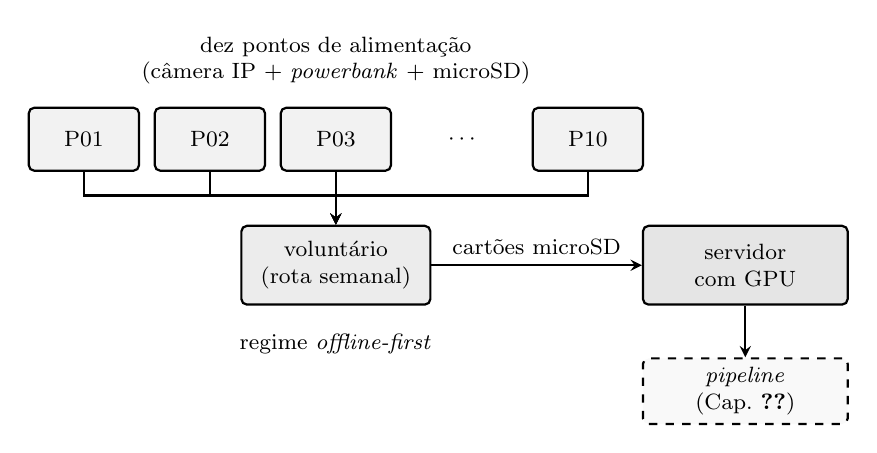
\begin{tikzpicture}[
      x=1cm, y=1cm,
      every node/.style={font=\footnotesize},
      pt/.style={draw, thick, rounded corners=2pt, fill=gray!10,
                 minimum width=1.4cm, minimum height=0.8cm, align=center},
      vol/.style={draw, thick, fill=gray!15, rounded corners=2pt,
                  minimum width=2.4cm, minimum height=1.0cm, align=center},
      srv/.style={draw, thick, fill=gray!20, rounded corners=2pt,
                  minimum width=2.6cm, minimum height=1.0cm, align=center},
      pipe/.style={draw, thick, dashed, fill=gray!5, rounded corners=2pt,
                   minimum width=2.6cm, minimum height=0.8cm, align=center},
      flow/.style={->, >=stealth, thick}
    ]
    % Pontos P01..P10
    \node[pt] (p1)   at (0.0,2.6) {P01};
    \node[pt] (p2)   at (1.6,2.6) {P02};
    \node[pt] (p3)   at (3.2,2.6) {P03};
    \node     (pdot) at (4.8,2.6) {$\cdots$};
    \node[pt] (p10)  at (6.4,2.6) {P10};

    % Rótulo do conjunto
    \node[align=center] at (3.2,3.6)
      {dez pontos de alimentação\\
       (câmera IP + \textit{powerbank} + microSD)};

    % Voluntário
    \node[vol] (vol) at (3.2,1.0) {voluntário\\(rota semanal)};

    % Servidor
    \node[srv] (srv) at (8.4,1.0) {servidor\\com GPU};

    % Pipeline
    \node[pipe] (pipe) at (8.4,-0.6) {\textit{pipeline}\\(Cap.~\ref{cap:pipeline})};

    % Fluxos pontos -> voluntário
    \foreach \n in {p1,p2,p3,p10}{
      \draw[flow] (\n.south) -- ++(0,-0.3) -| (vol.north);
    }

    % Voluntário -> servidor
    \draw[flow] (vol.east) -- node[above] {cartões microSD} (srv.west);

    % Servidor -> pipeline
    \draw[flow] (srv.south) -- (pipe.north);

    % Rótulo do regime
    \node[align=center] at (3.2,0.0) {regime \textit{offline-first}};
  \end{tikzpicture}
  \caption[Arquitetura recomendada de aquisição e fluxo de dados até o pipeline.]
  {Arquitetura de aquisição recomendada para os dez pontos de alimentação do Campus 2. Cada ponto opera com câmera IP adaptada, \textit{powerbank} e cartão microSD industrial em regime \textit{offline-first}. Os cartões são recolhidos em rota semanal pelos voluntários da AEX Gatos do C2 e levados ao servidor com GPU, onde alimentam o \textit{pipeline} de visão computacional do Capítulo~\ref{cap:pipeline}, executado em lote.}
  \label{fig:arquitetura-recomendada}
  \fonte{Elaborado pelo autor.}
\end{figure}


A escolha por tipologia única não exclui as demais tipologias do projeto, reserva-as a finalidades específicas. As \textit{trail cameras} alimentadas por baterias permanecem como referência comparativa para validação experimental nos pontos sem insolação adequada. Conjuntos SBC com NPU mantêm-se como referência para etapas do \textit{pipeline} em borda, podendo ser implantados em uma ou duas unidades-piloto para avaliar o ganho de descarte antecipado de quadros sem animal. Os módulos baseados em microcontrolador ficam reservados a redes densas de prova de conceito. Essas tipologias entram no projeto como unidades experimentais paralelas, não substituindo a tipologia padronizada nos dez pontos operacionais. O detalhamento de \textit{datasheets}, dimensionamento de \textit{powerbanks} e cartões microSD, classes de proteção, ângulos de montagem e pilotos paralelos é mantido no Apêndice~\ref{ap:hardware}.


A adoção da câmera IP em modo \textit{offline} como tipologia única tem três consequências diretas para o Capítulo~\ref{cap:pipeline}. O \textit{pipeline} pressupõe a chegada de quadros em formato comprimido (JPEG ou H.264), sem metadados de pré-inferência embarcada, e concentra a capacidade de processamento integralmente em servidor. A uniformidade da tipologia simplifica o estágio de normalização e calibração, que passa a tratar variações de geometria e iluminação entre pontos sem precisar absorver heterogeneidade adicional vinda do próprio sensor. A cadência de chegada de dados é determinada pelo ciclo logístico de retirada de cartões e troca de \textit{powerbanks}, com periodicidade semanal ou quinzenal, o que estrutura o \textit{pipeline} em regime de lote sobre janelas históricas e dispensa hipóteses sobre latência de transmissão. A presença de fauna não-alvo, herdada da Seção~\ref{sec:cap2-pontos}, mantém a classificação multiespécie como pré-requisito funcional da re-ID.
